In our solution we import the initial contours by loading a black and
white image and analyse it to create the SDF matching it. 

To generate the SDF we start by constructing two Cartesian grids of
the same sizes as the image. One to hold the distances to the contour
on the outside of the object, and one for the inside. The ``outer
grid'' is populated with (0,0) if the pixel is dark and
(``infinite'',``infinite'') if it's white, and opposite for the inner
grid. This way each entry in the grid has a vector.

The next step is to calculate the actual distances to the iso-contour
for each pixel. We first traverse the image pixel by pixel from top
left corner to the lower right. For each row in the grid we go from
left to right and for each pixel calculate the length of our vector in
this entry against all the neighboring pixels vectors. The distance is
the vector length of the vector created with the x,y values in the
grid. If the distance in a neighbor, plus the offset to the current
pixel, is smaller than the one already in the given pixel, it is
substituted with the new and smaller one. This way we keep the 0
values inside the object, and use this value to propagate out to the
pixels we visit afterwards.

\begin{figure}[htb]
  \centering
  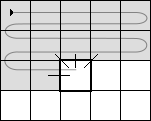
\includegraphics[scale=0.8]{imgs/sean-mikkel.png}
  \caption{Building the Signed Distance Function table, pixel by pixel from an image.}
  \label{build_sdf:fig:sean-mikkel}
\end{figure}

When we reach the end of a row we go back again in the same row, and
now check the same pixels, this time checking the pixel to the right
of it, also filling out distances to the left of objects. The
navigation in the grid can be seen in
figure \vref{build_sdf:fig:sean-mikkel}.

We now have distances below all objects in the image. If we now run
the same pass again, just starting from the bottom and moving up, we
have a vector at each pixel with the offset to the nearest contour.

Doing the same with the opposite starting values will create a
distance grid with the values from inside objects in the
image. Subtracting the distance of the vectors in the second grid
from the first will give us an $\phi$-value for each pixel, and we can
now save these as our $\phi$.

This SDF will have to be reinitialized numerous times afterwards to
complete it, as the contour should be a smooth line instead of a 1-pixel
wide line following pixels completely. This will be covered in section \vref{sec:reinitialize}. When the SDF has been reinitialized it will become as smooth as the one depicted in figure \vref{introduction:fig:cartesiangrid}.



